\documentclass[11pt]{article}
% Defining all packages that are used in this document
\usepackage[utf8]{inputenc}
\usepackage[english]{babel} % Change this to norwegian if report is written in norwegian
\usepackage{amsmath}   % Package for math files
\usepackage{parskip}   % No indent, but instead paragraphs
\usepackage{graphicx}  % Place figures
\usepackage{caption}   % Place captions in tables and figures
\usepackage{subcaption}% 
\usepackage{subfiles}  % 
\usepackage[T1]{fontenc} 
\usepackage[euler]{textgreek} % To get greek letters as we know them
\usepackage{amssymb}   % 
\usepackage{placeins}  % \FloatBarrier so figures can't float beyond some point in text
\usepackage{fullpage}  % Uses more of the page
\usepackage{float}     % Able to make figures and tables float \begin{figure}[H] to keep them HERE
\usepackage[version=4]{mhchem} % \ce{} to write chemical eq.
\usepackage{siunitx}   % Ex: \si{\meter\per\square\second}
\usepackage{booktabs}  % Behind-the-scenes optimization of tables. \toprule, \midrule, \bottomrule
\usepackage{hyperref}  % Ability to click on references like equations, figures, sections etc. \ref{eq:my_eq} clickable
\hypersetup{
    colorlinks,
    citecolor=black,
    filecolor=black,
    linkcolor=black,
    urlcolor=black
}
\usepackage[autolinebreaks,useliterate,numbered]{mcode} % Ability to paste smooth MATLAB code

\title{
    Title of Report - Make This Appealing and Remember Rules for Capitalization
    }
\author{
    Smith, J.\footnote{john@example.com}, Brown, J.\footnote{james@example.com}, \\
    Greenwood, A. \footnote{arthur@example.com}, Graham, T.\footnote{tim@example.com}
}
\date{
    Day Month, Year (not \textbackslash today)\\
    Example: 26 April, 2017
}

\begin{document}
\maketitle
\begin{abstract}
    This section should contain a short and concise way of describing all parts of the report. It should be a summary of the introduction, what has been done and what you have found.
\end{abstract}
\pagenumbering{gobble} % Turn off page numbering
\newpage
\tableofcontents
\newpage
\pagenumbering{arabic} % Turn on normal pagenumbering
%%%%%%%%%%%%%%%%%%%%%%%%%%%%%%%%%%%%%%%%%%%%%%%%%%%%%%%%%%
% Main contents - Do NOT write your text in main.tex! Use                     the tex files in the folders below
\section{Introduction}
\label{sec:introduction}
\FloatBarrier % Now figures cannot float above section title
This section should concentrate on what has previously been done in the field of research, so that it incentivizes the experiment. Why is there a need to gain knowledge on this specific field, and what motivates you to conduct the experiment? Often the introduction lists up a lot of historical facts and previous reports, and then it presents the topic for the report. The section is here for make a smooth transaction over to what you will be covering later on. It may be a good idea to present figures to back up your claims as done in figure \ref{fig:intro_co2}. Never post jpg, jpeg or bmp files in figures, but try to stick to png or eps format. Even though you have presented the figure in this text, the caption on the figure must still be able to present the information alone independent of this text! It should also be placed BENEATH the actual figure. Also remember to always write passive, i.e no personal pronouns (I, you, he, we, you, they). It is recommended that you learn Mendeley for managing your references that has great support in Sharelatex. Upper left corner $\rightarrow$ Menu $\rightarrow$ Mendeley inserts your whole personal library into the document, so that you don't have to worry about formatting your references correctly. \LaTeX does that for you.
% Historical chart of CO2 emissions
\begin{figure}[htb] % Here, top, bottom priority list
    \centering
    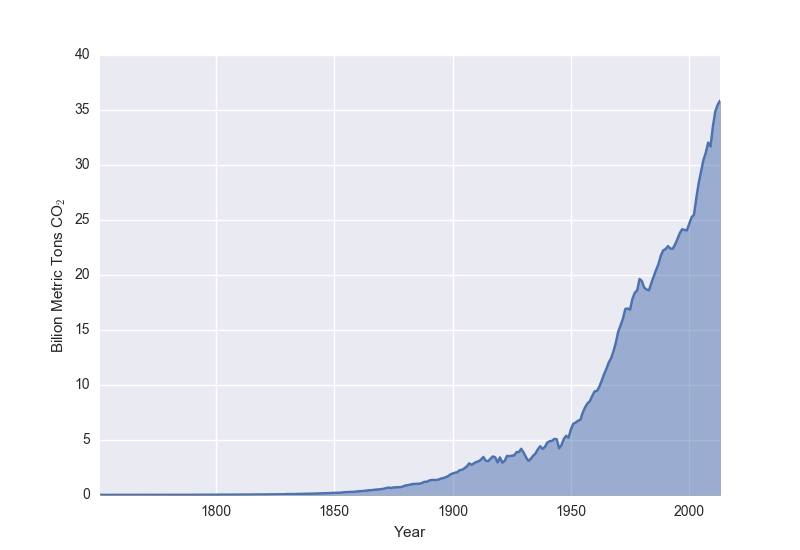
\includegraphics[scale=0.45]{Introduction/figures/Historic_CO2_Emission}
    \caption{This text should be able to stand alone independent of text outside figure!}
    \label{fig:intro_co2}
\end{figure}
\section{Problem Description}
\label{sec:problem_description}
For a lab report you should dedicate this section to introducing necessary theory that you will later use to develop results and calculate necessary values, and present the experimental setup. It is probably a better idea in this case to structure your report in a section Background Theory and another section Experimental, where you should present how you have proceeded to produce your results in the latter of those two. For a report that is more theoretical, you could rather use the section Problem Description where you describe the experimental setup and the model equations you have developed for the particular system. This could for instance be a simplified steady state system for mass flows, as in \ref{eq:mass_balance}.
% Mass balance for a stationary system
\begin{equation}
    \label{eq:mass_balance}
    \hat{m}_{in} = \hat{m}_{out}
\end{equation}
Remember to explain all symbols that have been presented in the equations in text. In equation \ref{eq:mass_balance} $\hat{m}_{in}$ is mass flow into the system and $\hat{m}_{out}$ is mass flow out of the system. All symbols should appear in the text exactly as they do in the equations, hence the math shift is used to present the mass flows.
An example of an equation with fractions
\begin{equation}
    \frac
    {3\alpha + 2\alpha^2}
    {7\omega^3}
\end{equation}
An example of subequations
\begin{subequations}
    \label{eq:equation_set1}
    \begin{equation}
        \label{eq:equation_set1_a}
        \hat{m}_{1} = \hat{m}_{2} + \hat{m}_{3}
    \end{equation}
    \begin{equation}
        \label{eq:equation_set1_b}
        \hat{m}_{3} = \hat{m}_{2} + \hat{m}_{4}
    \end{equation}
\end{subequations}
You can reference the equation set \ref{eq:equation_set1} and its corresponding subequation \ref{eq:equation_set1_a} and \ref{eq:equation_set1_b}.
It is good practice to include a picture of the setup as in figure \ref{fig:setup}.
\begin{figure}[htb]
    \centering
    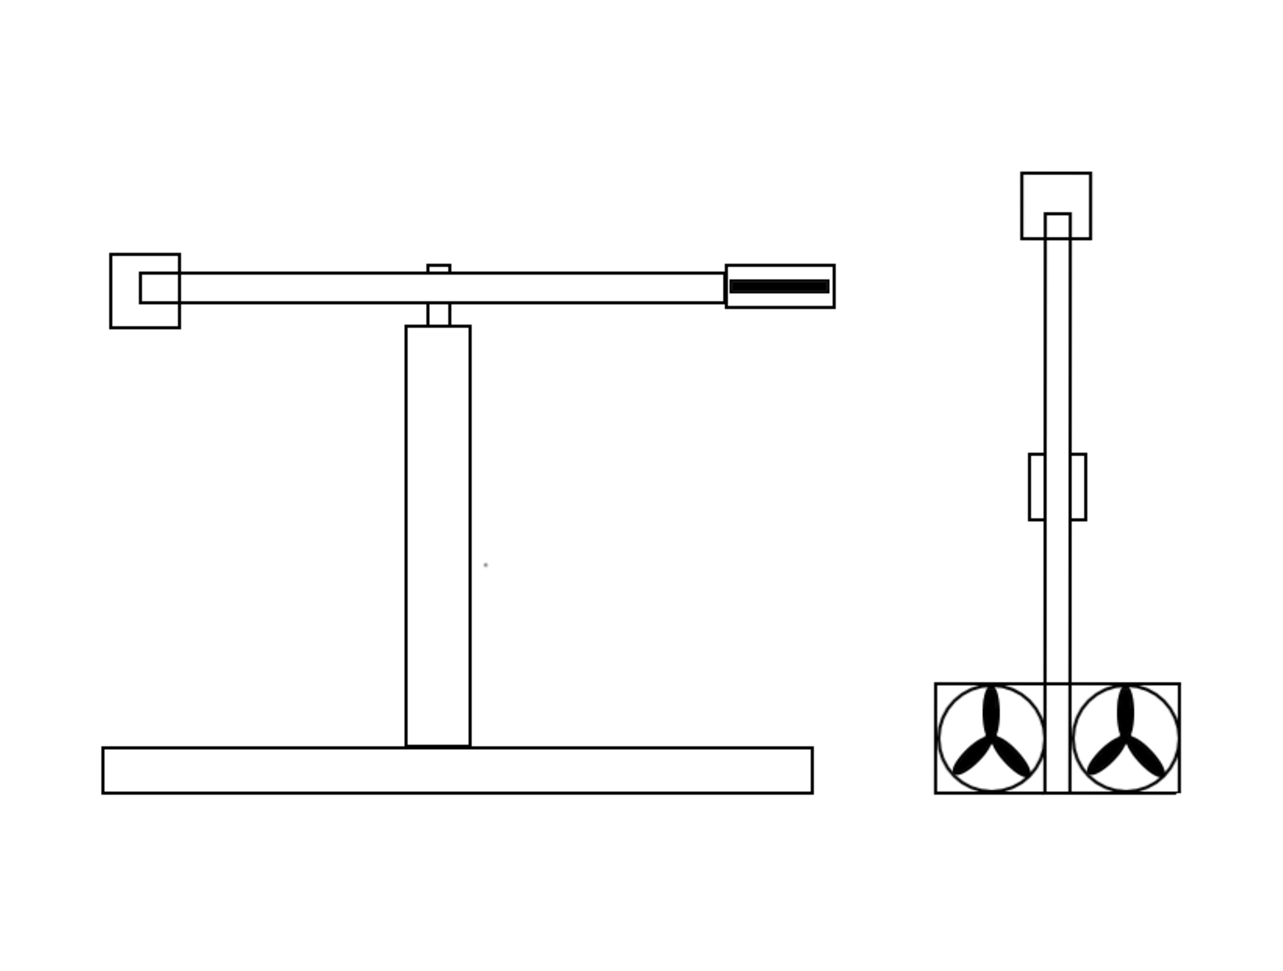
\includegraphics[scale=0.5]{Problem_description/figures/helikopter.eps}
    \caption{The figure shows the setup of the experiment performed.}
    \label{fig:setup}
\end{figure}

\section{Results}
\label{sec:results}
You should present all relevant information in this section objectively. There is no need to include calculations, that can be shown in appendix, (for instance as such: see appendix \ref{app:first_appendix}), but be sure that all measurements and end results are in the report. As a tool to make things easier to read, you could use tables as in \ref{tab:my_table}\cite{SICD}. You can refer to the appendix where you have done your calculations to back up that your end results are correct, and to keep the flow structure clean.
\begin{table}[htb]
    \centering
    \caption{The tables presents the standard enthalpy of formation and the standard entropy used to calculate the thermodynamics of the combustion of carbon.}
    \begin{tabular}{ccc} % all columns are centered. You can also use lll, rrr or any combination of the three
    \toprule
                    & $\Delta_fH^{\circ}$ [\si{\kilo\joule\per\mole}]  & $S{^\circ}$ [\si{\joule\per\kelvin\per\mole}] \\
    \midrule
        \ce{C}      &  140 & 201 \\
        \ce{O2}     &  103 & 104 \\
        \ce{CO2}    &  430 & 210 \\
    \bottomrule
    \end{tabular}
    \label{tab:my_table}
\end{table}
In table \ref{tab:my_table} all columns are centered. This is shown by the ccc tag inside the curly braces. You can also use lll, rrr, to create left aligned columns or right aligned columns respectively, or any combination of the three. The caption in tables should ALWAYS be on top of the actual table.
\FloatBarrier % Now the table doesn't flow over to any other sections
\section{Discussion}
\label{sec:discussion}
All your results should be presented by now, and all that remains is that you discuss them. You should always be critical of your results, and if they are not in correspondence with your theory presented in section \ref{sec:problem_description} this should be elaborated on! Why is there a mismatch between those two? What could have gone wrong and what do these non-correspondences imply? If there are undiscussed results, do not neglect them! It is easily seen and it doesn't look good in the report. Good reports really stand out from bad ones in this section and you can shine through if you have a well thought through reflection here.
\section{Conclusion}
\label{sec:conclusion}
The conclusion should, as the abstract, wrap up what you have found in the experiment. It should state what you have done and what you have found. The conclusion should only state what is obvious from the discussion in section \ref{sec:discussion}; no new information should arise here. The conclusion is the first place the reader will go looking if he wants to get an overview of the report. If it is interesting, he might read the rest. Be sure that the conclusion is short and concise, but do not omit important information. You have one shot at presenting your results: if you have done excellent work at the lab it doesn't matter if you are unable to present the results in an appealing way. The report is your only way of communicating and presenting your hard work.
\section*{List of Symbols}
\begin{table}[H]
\centering
\begin{tabular}{lll}
 \toprule
  \textbf{Symbol}   &\textbf{Unit}      &\textbf{Explanation}\\
  \midrule
    n               & \si{\mole}        & Amount of substance \\
    m               & \si{\kilo\gram}   & Mass \\
    H               & \si{\kilo\joule\per\mole} & Molar enthalpy \\
    S               & \si{\joule\per\kelvin\per\mole}   & Molar entropy \\
    G               & \si{\kilo\joule\per\mole} & Gibbs free energy \\
    A               & \si{\kilo\joule\per\mole} & Helmholtz free energy \\
  \bottomrule
  \end{tabular}
\end{table}

%%%%%%%%%%%%%%%%%%%%%%%%%%%%%%%%%%%%%%%%%%%%%%%%%%%%%%%%%%
% Bibliography
\newpage
\bibliographystyle{IEEEtran}
\bibliography{mendeley.bib}
%%%%%%%%%%%%%%%%%%%%%%%%%%%%%%%%%%%%%%%%%%%%%%%%%%%%%%%%%%
% Appendix
\appendix
\pagenumbering{roman}
\section{First Appendix}
\label{app:first_appendix}
\section{Second Appendix}
\section{Third Appendix}
\end{document}
